%  This section may be divided by subheadings. It should provide a concise and precise description of the experimental results, their interpretation as well as the experimental conclusions that can be drawn. 

\section{Results}

\if 0 This section may be divided by subheadings. It should provide a
concise and precise description of the experimental results, their
interpretation as well as the experimental conclusions that can be
drawn.

%%%%%%%%%%%%%%%%%%%%%%%%%%%%%%%%%%%%%%%%%%
\subsection{Subsection}
\subsubsection{Subsubsection}

Bulleted lists look like this:
\begin{itemize}[leftmargin=*,labelsep=4mm]
\item First bullet
\item Second bullet
\item Third bullet
\end{itemize}

Numbered lists can be added as follows:
\begin{enumerate}[leftmargin=*,labelsep=3mm]
\item First item
\item Second item
\item Third item
\end{enumerate}

The text continues here.

\subsection{Figures, Tables and Schemes}

All figures and tables should be cited in the main text as Figure 1,
Table 1, etc.

\begin{figure}[H]
  \centering %
\includegraphics[width=3cm]{./Figures/logo-mdpi}
  \caption{This is a figure, Schemes follow the same formatting. If
    there are multiple panels, they should be listed as: (\textbf{a})
    Description of what is contained in the first panel. (\textbf{b})
    Description of what is contained in the second panel. Figures
    should be placed in the main text near to the first time they are
    cited. A caption on a single line should be centered.}
\end{figure}   

\begin{table}[H]
  \caption{This is a table caption. Tables should be placed in the
    main text near to the first time they are cited.}  \small % Font
  size can be changed to match table content. Recommend 10 pt.
  \centering
  \begin{tabular}{ccc}
    \toprule \textbf{Title 1} & \textbf{Title 2} & \textbf{Title
      3}\\ \midrule entry 1 & data & data\\ entry 2 & data &
    data\\ \bottomrule
  \end{tabular}
\end{table}

\subsection{Formatting of Mathematical Components}

This is an example of an equation:

\begin{equation}
  \mathbb{S}
\end{equation}

%% If the documentclass option "submit" is chosen, please insert a blank line before and after any math environment (equation and eqnarray environments). This ensures correct linenumbering. The blank line should be removed when the documentclass option is changed to "accept" because the text following an equation should not be a new paragraph. 
Please punctuate equations as regular text. Theorem-type environments
(including propositions, lemmas, corollaries etc.) can be formatted as
follows:
%% Example of a theorem:
\begin{Theorem}
  Example text of a theorem.
\end{Theorem}
The text continues here. Proofs must be formatted as follows:

%% Example of a proof:
\begin{proof}[Proof of Theorem 1]
  Text of the proof. Note that the phrase `of Theorem 1' is optional
  if it is clear which theorem is being referred to.
\end{proof}
The text continues here.  \fi
%%%%%%%%%%%%%%%%%%%%%%%%%%%%%%%%%%%%%%%%%%

\subsection{Performance Assessment}

At the competition, the Vanderbilt AGSE was able to complete the
sample retrieval process in approximately $4.5$ minutes. The recovery
process, as shown in Figure \ref{fig:AGSE_Operation}, was successful,
with payload and rocket bay recognition occurring quickly and
efficiently. The AGSE was able to grasp the payload using only two of
its four padded end effector phalanges, and successfully deposited the
payload within the rocket bay. This operation received high marks from
the NASA officials and earned the competition's \emph{Autonomous
  Ground Support Equipment Award}.

\begin{figure}[t]
  \centering
  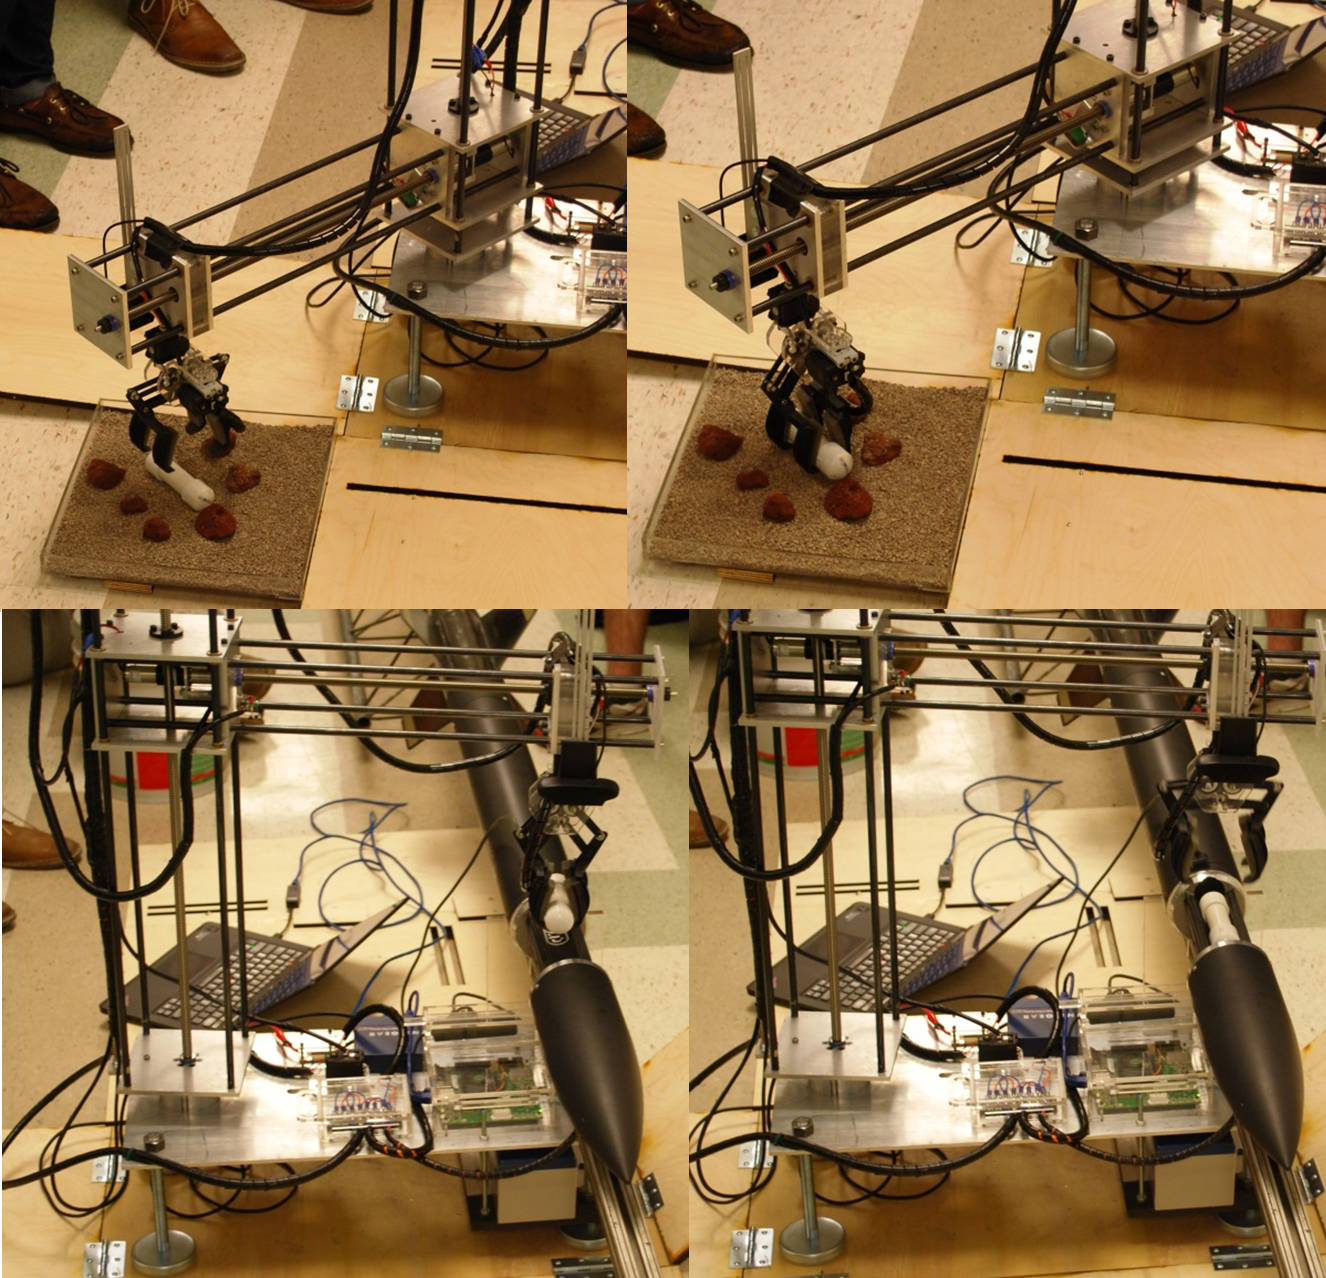
\includegraphics[width=0.75\linewidth]{Figures/AGSE_Operation.png}
  \caption{AGSE Calibration and Testing}
  \label{fig:AGSE_Operation}	
\end{figure}

System robustness was validated on the day of competition when a key
component failed and was able to be quickly replaced with a different
part with no detriment to system performance. The Dynamixel AX-12A
servo controlling the base rotational degree of freedom of the AGSE
suffered an irreparable failure of its gearbox and had to be removed
from the robot. A backup of the servo was not readily available, and a
different model servo by the same company had to be swapped in
instead.  This new model, a Dynamixel MX-28T, while having similar
performance as the old servo, had a different communication protocol
and mounting footprint, as well as a more complex control scheme.

The component-based nature of ROSMOD allowed quick modifications of
the business logic of the \emph{rotation\_controller} component to
update the system to use the new hardware.  The new control scheme was
quickly implemented and the control software was updated to account
for the new physical placement of the servo due to its different
mounting footprint. After these modifications were made, the AGSE was
able to perform at its optimal level during its part of the
competition.

